\documentclass{beamer}

%\usetheme{Malmoe}
%\usetheme{Szeged}
%\usepackage{beamerthemesplit}

\usefonttheme{serif} 
%\usepackage[normalem]{ulem}
%\usepackage[english]{babel}
%\usepackage[latin1]{inputenc}
%\usepackage{times}
%\usepackage[T1]{fontenc}

\usecolortheme{dolphin}

\newtheorem{remark}{Remark}

\usepackage{listings}
\usepackage{fancyvrb}
\lstnewenvironment{newcode}{\lstset{language=Haskell,basicstyle=\scriptsize,escapechar=\@}}{}
\newcommand{\ttcode}[1]{{\color{red}{\tt{#1}}}}

\setbeamertemplate{navigation symbols}{}

\newenvironment{codeblock}[1][.8]{%
\begin{columns}
\begin{column}{#1\linewidth}
\begin{exampleblock}{}}{%
\end{exampleblock}
\end{column}
\end{columns}} 

\newenvironment{execblock}[1][.8]{%
\begin{columns}
\begin{column}{#1\linewidth}
\begin{block}{}}{%
\end{block}
\end{column}
\end{columns}} 

\def\slideskip{\vskip 0.1in}
\def\frameskip{\vskip 0.1in}

\usepackage{hyperref}

\def\@fnsymbol#1{\ensuremath{\ifcase#1\or *\or \dagger\or \ddagger\or
   \mathsection\or \mathparagraph\or \|\or **\or \dagger\dagger
   \or \ddagger\ddagger \else\@ctrerr\fi}}
\renewcommand{\thefootnote}{\fnsymbol{footnote}}   
\newcommand{\forget}[1]{}
\title{{\tt mov} is Turing Complete}
\subtitle{CS4440 Spring 2017}
\author[]{Stephen Dolan\footnote{...as told by Bill Harrison}}
\date{\today}

\begin{document}

\frame{\titlepage}

%%%%%%%%%%%%%%
%%%%%%%%%%%%%%
%%%%%%%%%%%%%%
%%%%%%%%%%%%%%
\section{Introduction}

\begin{frame}[fragile]
\frametitle{Introduction: Turing Completeness}

\begin{itemize}
\item Alan Turing (1912-54) was an English logician who, among his many accomplishments, invented a notion of what ``computable function'' means.
\pause
\item ``Turing Machines'' are abstract machines (we'll define them later) with a particular instruction set
\begin{itemize}
\item Function is \emph{Turing computable} means that you can program a Turing machine that computes that function
\end{itemize}
\pause
\item Other definitions of computability used $\lambda$-calculus (Haskell Curry) and register machines (Johan von Neumann).

\pause 
\item Languages are said to be \emph{Turing complete} when you can write a Turing machine simulator in the language.
\pause

\item This is what Hovav Schacham et al. are showing in ``Geometry of Innocent Flesh...'': 
\begin{itemize}
\item Can simulate a Turing complete language with gadgets, so ROP is Turing complete.
\end{itemize}

\end{itemize}
\end{frame}

\begin{frame}[fragile]
\frametitle{{\tt mov} is Turing complete}

\begin{itemize}
\item The \verb+x86+ instruction set is, to put it mildly, \emph{complex}
\pause
\item \verb+mov+ instruction has quite a few addressing modes, allowing it to perform complex memory loads/stores and register transfers

\pause
\begin{itemize}
\item ...\emph{but} it has no means of conditional branching or comparison
\item ...so sequences of \verb+mov+ instructions always terminate.
\end{itemize}
\pause

\item Dolan shows that, with precisely \emph{one} unconditional jump, one can simulate a Turing machine with only x86 \verb+mov+ instructions!
\pause

\item Relevance to Malware Analysis?
\pause
\begin{itemize}
\item There are \emph{many} modes of computing with {\tt x86} beyond those intended by Intel!
\pause
\item These computing modes are highly obfuscated:
\begin{itemize}
\item How do you know that ROP execution is being performed? How do you comprehend what a sequence of \verb+mov+ instructions does?
\end{itemize}
\end{itemize}

\end{itemize}

\end{frame}

%%%%%%%%%%%%%%
%%%%%%%%%%%%%%
%%%%%%%%%%%%%%
%%%%%%%%%%%%%%
\section{Machine Model}

\begin{frame}[fragile]
\frametitle{Machine Model}

\begin{itemize}
\item Using just the following instructions and one unconditional jump, can simulate a Turing machine:

\begin{center}
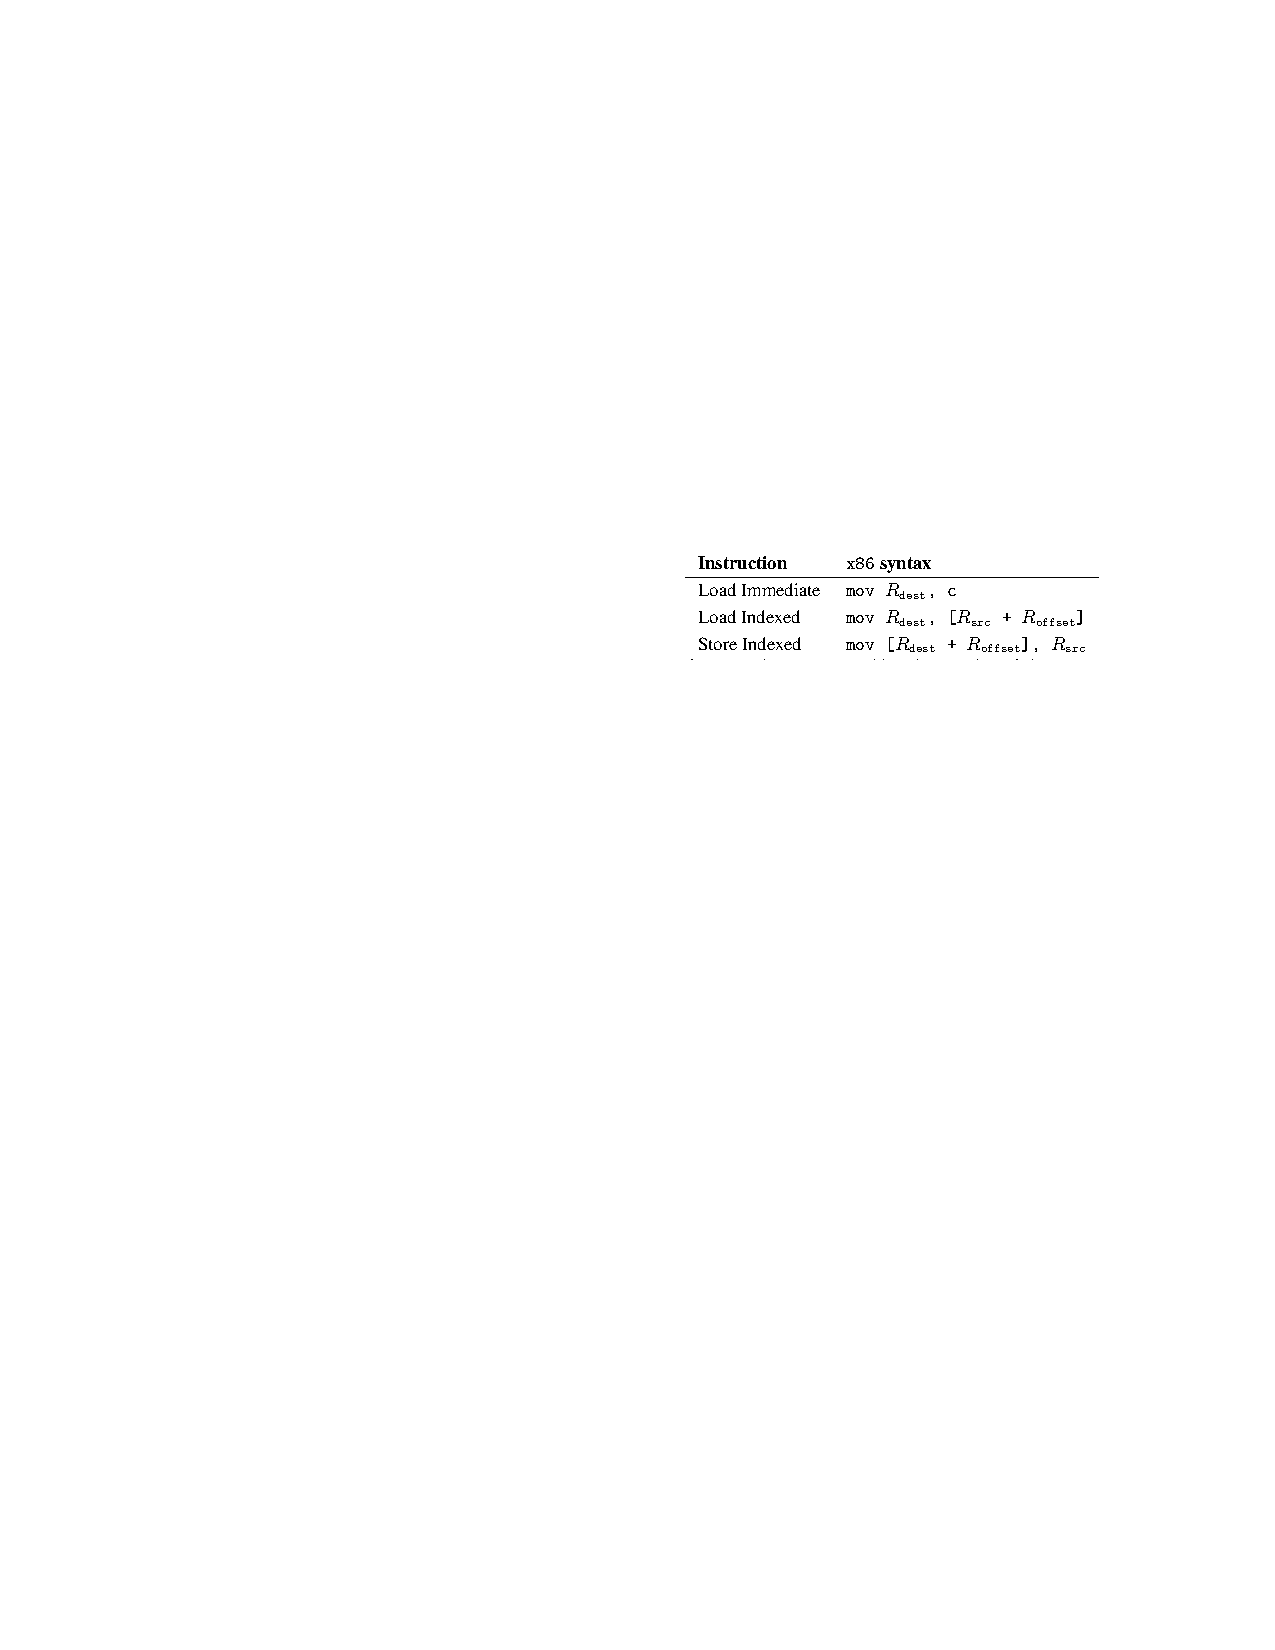
\includegraphics[scale=0.99]{figures/x86instructions}
\end{center}
\pause
\item x86 format: $\mathtt{mov~ R_{dst},~ R_{src}}$
\pause
\item Can define shorthand. E.g., \Verb+mov Rd,[Rs]+ is:
\begin{Verbatim}
mov X,0
mov Rd,[Rs + X] -- typo in paper here.
\end{Verbatim}

\end{itemize}
\end{frame}

%%%%%%%%%%%%%%
%%%%%%%%%%%%%%
%%%%%%%%%%%%%%
%%%%%%%%%%%%%%
\section{Comparisons and Conditionals}

\begin{frame}[fragile]
\frametitle{Comparisons: \Verb+Ri+ = \Verb+Rj+?}

\begin{itemize}
\item Say you have two pointers, \Verb+Ri+ and \Verb+Rj+, and you want to know if they point to the same object
\pause

\item Assume \Verb+0+ and \Verb+1+ represent false and true, resp. After this code chunk is executed, what value is in \Verb+Rk+?
\begin{Verbatim}
mov [Ri], 0
mov [Rj], 1
mov Rk,[Ri]
\end{Verbatim}
\pause
\item Here's the result:
\[
\mathtt{Rk} = 
\left\{\begin{array}{lcl}
\mathtt{1} && \mathtt{Ri} = \mathtt{Rj}
\\
\mathtt{0} && \mathtt{Ri} \neq \mathtt{Rj}
\end{array}\right.
\]
\end{itemize}
\end{frame}

\begin{frame}[fragile]
\frametitle{Comparisons: \Verb+Ri+ = $N$?}

\begin{itemize}
\item Assuming the contents of \Verb+N+ is $N$
\begin{Verbatim}
mov X, [Ri]
mov [N], 0
mov [Ri], 1
mov Rj, [N]
mov [Ri], X
\end{Verbatim}

\pause
\item Here's the result:
\[
\mathtt{Rj} = 
\left\{\begin{array}{lcl}
\mathtt{1} && \mathtt{Ri} = N
\\
\mathtt{0} && \mathtt{Ri} \neq N
\end{array}\right.
\]
\end{itemize}

\end{frame}

%%%%%%%%%%%%%%
%%%%%%%%%%%%%%
%%%%%%%%%%%%%%
%%%%%%%%%%%%%%
\section{Representing Turing Machines}

\begin{frame}[fragile]
\frametitle{Defining Turing Machines}

\begin{center}
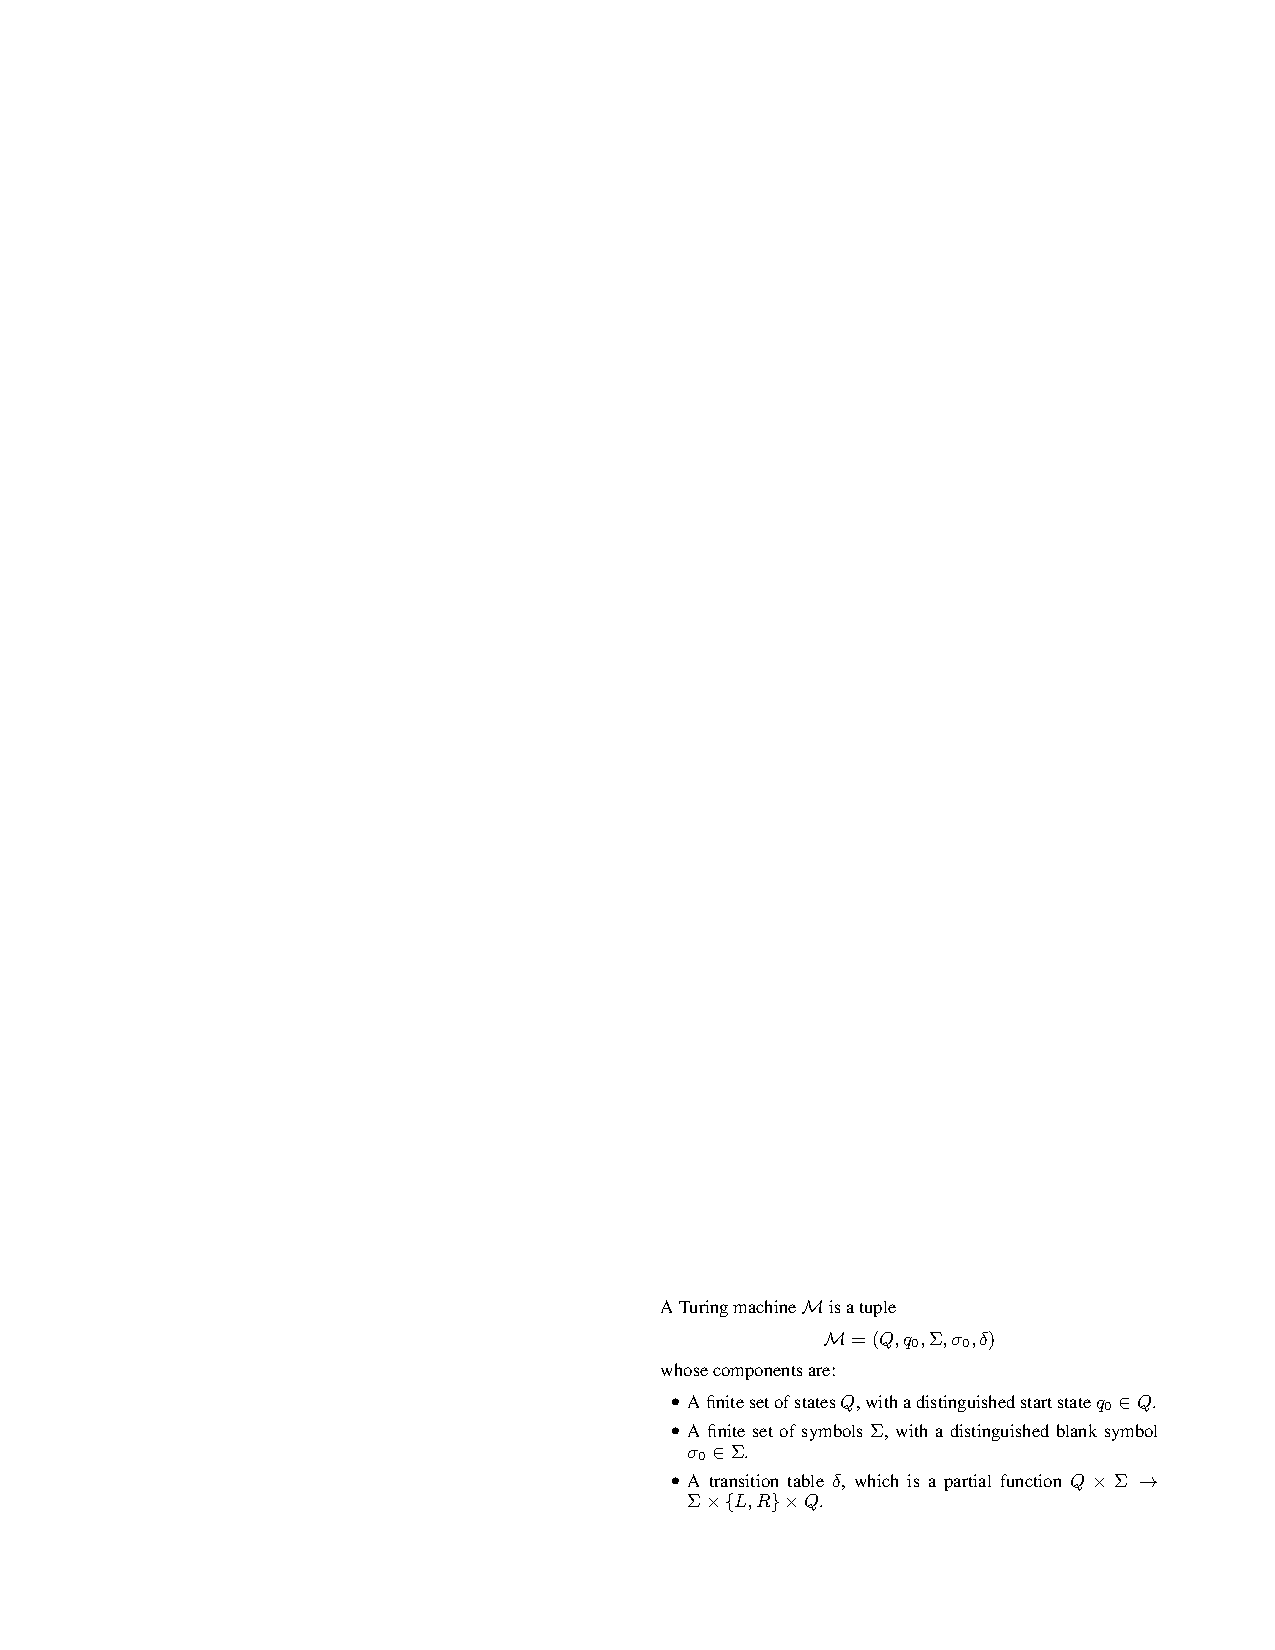
\includegraphics[scale=1.2]{figures/TuringMachine}
\end{center}

\end{frame}


\begin{frame}[fragile]
\frametitle{Representation of a Turing Machine}

\begin{center}
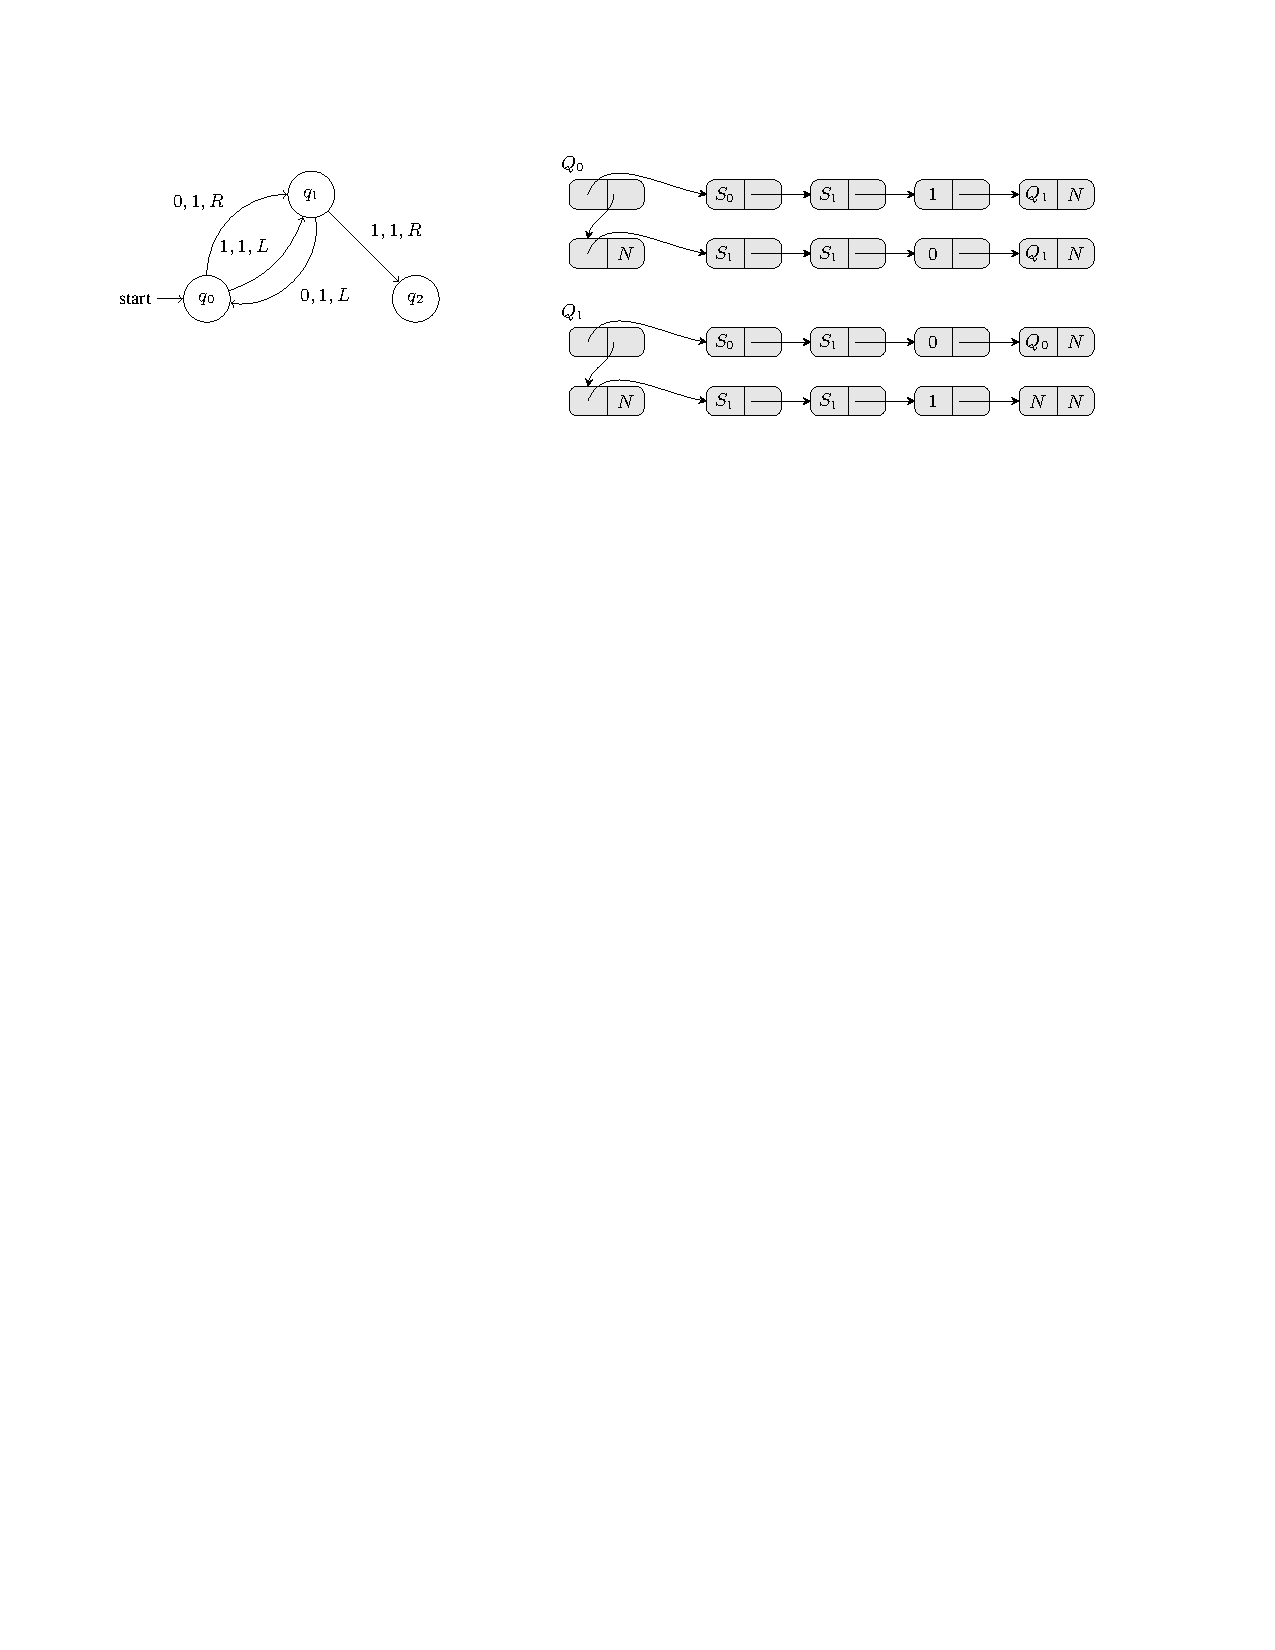
\includegraphics[scale=0.6]{figures/TMrepresentation}
\end{center}
\begin{columns}
\begin{column}{2.35in}
\begin{itemize}
\item Above is a state machine repr. 
\pause
\item Transition $q_0 \longrightarrow^{0,1,R} q_1$  means
that $\delta (q_0,0) = (1,R,q_1)$
\pause
\item English: if you're in $q_0$ and you see the $0$ symbol, replace it with $1$, go $R$, and enter state $q_1$
      \pause
\end{itemize}
\end{column}
\begin{column}{2.35in}
\begin{itemize}
\item Above encodes $\delta$ in memory
\pause
\item $S_0, S_1$ addresses of cells containing $0$ \& $1$
\pause
\item Top line represents $q_0 \longrightarrow^{0,1,R} q_1$
\item Confusingly, $1$ and $0$ represent $R$ and $L$, resp.

\end{itemize}
\end{column}
\end{columns}
\end{frame}
%%%%%%%%%%%%%%
%%%%%%%%%%%%%%
%%%%%%%%%%%%%%
%%%%%%%%%%%%%%
\section{Comparisons and Conditionals}

%\begin{frame}[fragile]
%\frametitle{}
%
%\begin{center}
%\includegraphics[scale=0.5]{figures/}
%\end{center}
%\end{frame}

%%%%%%%%%%%%%%
%%%%%%%%%%%%%%
%%%%%%%%%%%%%%
%%%%%%%%%%%%%%
\section{Simulating a Turing Machine}

%\begin{frame}[fragile]
%\frametitle{}
%
%\begin{center}
%\includegraphics[scale=0.5]{figures/}
%\end{center}
%\end{frame}

%%%%%%%%%%%%%%
%%%%%%%%%%%%%%
%%%%%%%%%%%%%%
%%%%%%%%%%%%%%
%\section{Register Use}
%
\begin{frame}[fragile]
\frametitle{Simulator Structure}

\begin{center}
\begin{verbatim}
start:
  mov X,[T]  ;; get transition
  mov X,[X]  ;; get trigger symbol
  mov Y,[S]  ;; get current symbol
  mov [Y],0  ;; compare symbols
  mov [X],1
  mov M,[Y]
      ...snip...
  jump start
\end{verbatim}
\end{center}
\begin{itemize}
\item There are several registers (e.g., $\mathtt{X, T, N}$, etc.) that maintain the state of the simulator
\end{itemize}
\end{frame}

\begin{frame}[fragile]
\frametitle{Summary \& Conclusions}

\begin{itemize}
\item Paper gives detailed description of a Turing Machine simulator
\pause
\begin{itemize}
\item ...and the details are, well, \emph{very detailed}
\end{itemize}
\pause
\item Question remains: is this merely a curiosity?
\begin{itemize}
\item Basis of a useful obfuscation technique?
\item Pragmatics of the idea are unexplored (not the point of the paper)
\end{itemize}
\end{itemize}
\end{frame}
%%%%%%%%%%%%%%
%%%%%%%%%%%%%%
%%%%%%%%%%%%%%
%%%%%%%%%%%%%%
\section{Discussion}

%\begin{frame}[fragile]
%\frametitle{}
%
%\begin{center}
%\includegraphics[scale=0.5]{figures/}
%\end{center}
%\end{frame}



\end{document}
    
